% Preamble
% Compile with XeLateX

\documentclass[11 pt,oneside,a4paper,titlepage]{article}
\usepackage{preamble}
\graphicspath{{./images/}} % path to the images
%%%%%%%%%%%%%%%%%%%%%%%%%%%%%%%%%%%%%%%%%%%%%%%%%%%%%%%%%%%%%%%%%%%%%%%%%%%%%%%%%%%%%%
\begin{document}

\sidebar{sideBarColor!25}
\simpleheader{titleBackColor}{Riccardo}{Periotto}{Computer Scientist |  Autonomous Systems Engineer}{white}

% Start Minipages
\vspace*{3.49cm}% start 8 cm from the top of the page}
    \adjustbox{valign=t}{\begin{minipage}{7.3cm} % large 7.4 cm from the top
    \vspace*{1.2cm} % text starts 1cm under the top of the minipage
            
        % Picture
        \begin{center}
        \begin{tikzpicture}
            \node[
            circle,
            minimum size=\cvPictureWidth,
            path picture={
            \node at (path picture bounding box.center){
             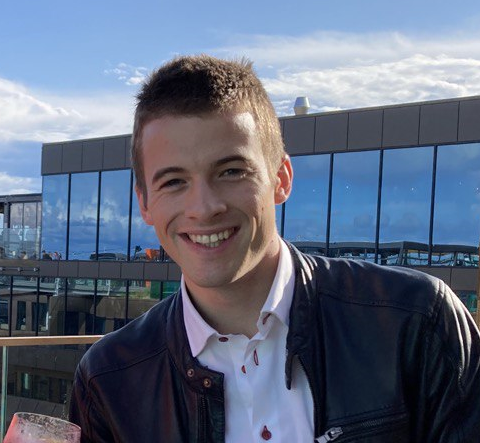
\includegraphics[width=\cvPictureWidth]{profile_stockholm.png}
             };
             }]
            {};
        \end{tikzpicture}
        \end{center}

        %%%%%%%%%%%%%%%%%%%%%%%%%%%%%%%%%%%%%%%%%%%%%%%%%%%%
        % Profile section
        \ruleline{\textbf{About me}}
        Driven by my passion for learning and technology, I embraced the ICT world in high school and delved into the subject until I got my bachelor's degree in Computer Science. After that, I worked in the field for one year and finally graduated in Autonomous Systems from a double degree program two years later. Since then, I have been working as a Software Engineer for robotics in Munich, where I contribute to simplifying the application of AI-driven solutions to industrial automation, particularly robotics.

        \vspace*{0.18cm}

        %%%%%%%%%%%%%%%%%%%%%%%%%%%%%%%%%%%%%%%%%%%%%%%%%%%
        % Contact Section
        \ruleline{\textbf{Personal information}}

        \begin{tikzpicture}[every node/.style={inner sep=0pt, outer sep=0pt}]

        \matrix [
        column 1/.style={anchor=center,contactIcon},
        column 2/.style={anchor=west,align=left,contactIcon},
        column sep=5pt,
        row sep=5pt] (contact) {
        
        \node{\faMale};
         & \node{Born on 15/09/1998};\\
        \node{\faEnvelope}; 
         & \node{\href{mailto:riccardo.periotto@gmail.com}{riccardo.periotto@gmail.com}};\\
        %& \node{Teknikringen 68A \\ 114 28 Stockholm, Sweden};\\
        \node{\faHome}; 
        & \node{
            \href{https://www.google.it/maps/place/38080+Carisolo+TN}
            {38080 Carisolo (TN), Italy }
        };\\
        % \node{\faMapMarker};
        % &\node{
        %     \href{https://www.google.it/maps/place/114+28+Stockholm}
        %     {Stockholm 114 28, Sweden}
        % };\\
        \node{\faLinkedinSquare}; 
        & \node{\href{https://www.linkedin.com/in/riccardoperiotto/}{riccardoperiotto}};\\
        \node{\faGithubSquare}; 
        & \node{\href{https://github.com/riccardoperiotto}{riccardoperiotto}};\\
        % \node{\faCar};
        % & \node{Driving License B};\\
        };
        \end{tikzpicture} 
        
        \vspace*{0.12cm}
        %%%%%%%%%%%%%%%%%%%%%%%%%%%%%%%%%%%%%%%%%%%%%%%%%%%
        % Languages
        \ruleline{\textbf{Languages}}
        \begin{tikzpicture}[every node/.style={inner sep=0pt, outer sep=0pt}]
        \matrix [
        column 1/.style={anchor=center,contactIcon},
        column 2/.style={anchor=west,align=left,contactIcon},
        column sep=5pt,
        row sep=5pt] (contact) {
        \node{\flag{italy.png}};
        & \node{Italian - Native Language};\\
        \node{\flag{england.png}};
        & \node{English - Professional Knowledge};\\
        \node{\flag{germany.png}};
        & \node{German - Basic Knowledge};\\
        };
        \end{tikzpicture} 
        
        \vspace*{0.12cm}
        
        %%%%%%%%%%%%%%%%%%%%%%%%%%%%%%%%%%%%%%%%%%%%%%%%%%%%
        % Programming Languages 
        \ruleline{\textbf{Programming languages}}
        \begin{center}
            \cvtag{C}\cvtag{C\#}\cvtag{C++}\cvtag{Java}\cvtag{Javascript}\cvtag{Maple}\cvtag{MATLAB}\cvtag{Python}\cvtag{R}
        \end{center}
        
        \vspace*{0.12cm}
        %%%%%%%%%%%%%%%%%%%%%%%%%%%%%%%%%%%%%%%%%%%%%%%%%%%%
        % Professional skills 
        \ruleline{\textbf{Hard skills}}
        \begin{center}
            \cvtag{Algorithms}\cvtag{Artificial Intelligence}\cvtag{Applied Estimation}\cvtag{Automatic Control}\cvtag{Data Structures}\cvtag{Databases \& SQL}\cvtag{Deep Learning}\cvtag{Dynamic Modeling}\cvtag{Full Stack Development}\cvtag{Machine Learning}\cvtag{Mechatronics}\cvtag{Object Oriented Programming}\cvtag{Robotics}\cvtag{Sensor Fusion}\cvtag{Software Engineering}
        \end{center}
    \end{minipage}} %
    \hfill 
%%%%%%%%%%%%%%%%%%%%%%%%%%%%%%%%%%%%%%%%%%%%%%%%%%%%%%%%%
%%%%% MAIN SECTION %%%%%%%%%%%%%%%%%%%%
    \adjustbox{valign=t}{\begin{minipage}{11.3cm}
        \vspace*{1cm}
        \section*{{\faGraduationCap} EDUCATION}           


        \vspace*{0.18cm}
            
        \MySectionNoPic{sep 2021-\\ nov 2023}{MSc Autonomous Systems}{EIT Digital}{Europe}{European double degree program focusing on new technologies, entrepreneurship, and business. \\

        First year: University of Trento (UniTN) \\
        Second year: Royal Institute of Technology (KTH)}

        \vspace*{0.21cm}
            
        \MySectionNoPic{sep 2017-\\jul 2020}{BSc Computer Science}{University of Trento}{Trento, Italy}{
        \\
        Main subjects: Algorithms, Software Engineering \\ 
        Grade: 110/110 with honours}

        \vspace*{0.21cm}

        \MySectionNoPic{sep 2014-\\jul 2017}{HS Computer Science}{ITT Marconi Rovereto}{Rovereto, Italy}{
        \\
        Main subjects: Programming, Network Systems\\ 
        Grade: 100/100 with honours}
        
        %%%%%%%%%%%%%%%%%%%%%%%%%%%%%%%%%%%%%%%%%%%%%%%%%%%
        % Work Experience
        \section*{{\faSuitcase} WORK EXPERIENCE (in the field of study)}

        \vspace*{0.18cm}

        \MySection{dec 2023-\\ ongoing }{agile_robots.png}{Software Engineer for Robotics}{\href{https://www.agile-robots.com/en/}{Agile Robots AG}}{Munich, Germany}{
        }{I'm working in the R\&D department on AgileCore, the company software platform facilitating the development and deployment of automation solutions.}

        \vspace*{0.18cm}

        \MySection{jan 2023-\\ jul 2023 }{ericsson.png}{Research Intern}{\href{https://www.ericsson.com/en}{Ericsson}}{Stockholm, Sweden}{
        }{I joined the research team to develop the research project for my master's degree. The result is a control algorithm for teleoperation aware of physical obstacles and network delays; more details can be found in the publication at the \href{https://arxiv.org/pdf/2403.18650}{link}.}
            
        \vspace*{0.18cm}
        
        \MySection{jan 2021-\\sep 2021}{polytec.jpg}{Software Engineer}{\href{https://polytec.bmgroup.com/}{BM Group Polytec S.p.A.}}{Borgo Chiese, Italy}{
        }{Development of cloud solutions for industrial plants. Video to the main project I worked on \href{https://youtu.be/XaXRUYPYLRw}{link}.}
            
        \vspace*{0.18cm}
        
        \MySection{oct 2019-\\feb 2020}{spaziodati.jpg}{Computer Science Intern}{\href{https://www.spaziodati.eu/}{SpazioDati S.r.l.}}{Trento, Italy}{
        }{I joined the company as an intern and developed my bachelor's degree project there. The main focus was to interface with the company's APIs and use their datasets in a web application.} 
        
        %%%%%%%%%%%%%%%%%%%%%%%%%%%%%%%%%%%%%%%%%%%%%%%%%%%
        % Information Technology Skills
        % (main one for saving space)
        \section*{{\faDesktop} TOOLS \& FRAMEWORK }
        \vspace*{-0.5cm}
        \begin{multicols}{2}    
        \begin{itemize}
        \footnotesize
            \item \textbf{.NET}: advanced
            \item \textbf{Django}: advanced
            \item \textbf{gRPC}: intermediate
            \item \textbf{Linux \& git}: advanced
            \item \textbf{Reach.js \& Vue.js}: intermediate    
            \item \textbf{ROS 2}: advanced
            \item \textbf{Unity}: intermediate
            \item[\vspace{\fill}]
        \end{itemize}
        \end{multicols}
        
        % \section*{{\faDesktop} PROFESSIONAL SKILLS}
        % 
        % \ITCcompetence{Software development}{
        % \textbf{.NET}: \textit{advanced}\\
        % \textbf{Node.js}: \textit{advanced}\\
        % \textbf{Unity}: \textit{intermediate}\\
        % }
        % 
        %  \ITCcompetence{ML/DL}{
        % \textbf{Scikit-learn}: \textit{intermediate}\\
        % \textbf{PyTorch}: \textit{intermediate}\\
        % }
        % 
        % \ITCcompetence{Others}{
        % \textbf{git}: \textit{advanced}\\
        % \textbf{ROS2}: \textit{beginner}\\
        % \textbf{MapleSim}: \textit{beginner}\\
        % }

         I live in a tourist area and have always done \textbf{seasonal jobs}. I do my best to complete what I commit to and, sometimes, I am even far too meticulous; this is why my scout \href{https://it.wikipedia.org/wiki/Totem_(nome_scout)}{totem} is \textit{Precise Hedgehog}. I love sports, particularly climbing, running, and snowboarding: I don't do them competitively, but I am honestly addicted to them!      

        \vspace*{0.18cm}
        Updated version of this document available at: \href{https://riccardoperiotto.github.io/CV_RiccardoPeriotto.pdf}{CV\_RiccardoPeriotto}. \\
        Date: \today.
    \end{minipage}} %
\end{document}
